\chapter{Introducción}\label{cap1}

\section{Introducción}
\textbf{La Inteligencia Artificial (IA)} ha ido integrándose de forma progresiva en múltiples aspectos de la vida cotidiana. Aunque sus orígenes se puedan trazar a hace varias décadas, no ha sido hasta los últimos años cuando el público general ha empezado a interactuar de forma consciente con sistemas inteligentes. Algunos ejemplos son los vehículos autónomos como los de Tesla, o los sistemas de clasificación automática de fotografías en dispositivos móviles.

Sin embargo, el mayor punto de inflexión en la percepción social de la IA ha sido la aparición de los \textit{Large Language Models} (LLM), cuyo impacto ha sido especialmente notorio a través de interfaces conversacionales como ChatGPT. Para ilustrar su crecimiento, se muestra a continuación la evolución del número de consultas diarias a este tipo de sistemas:

\vskip 0.15cm
\begin{figure}[H]
    \centering
    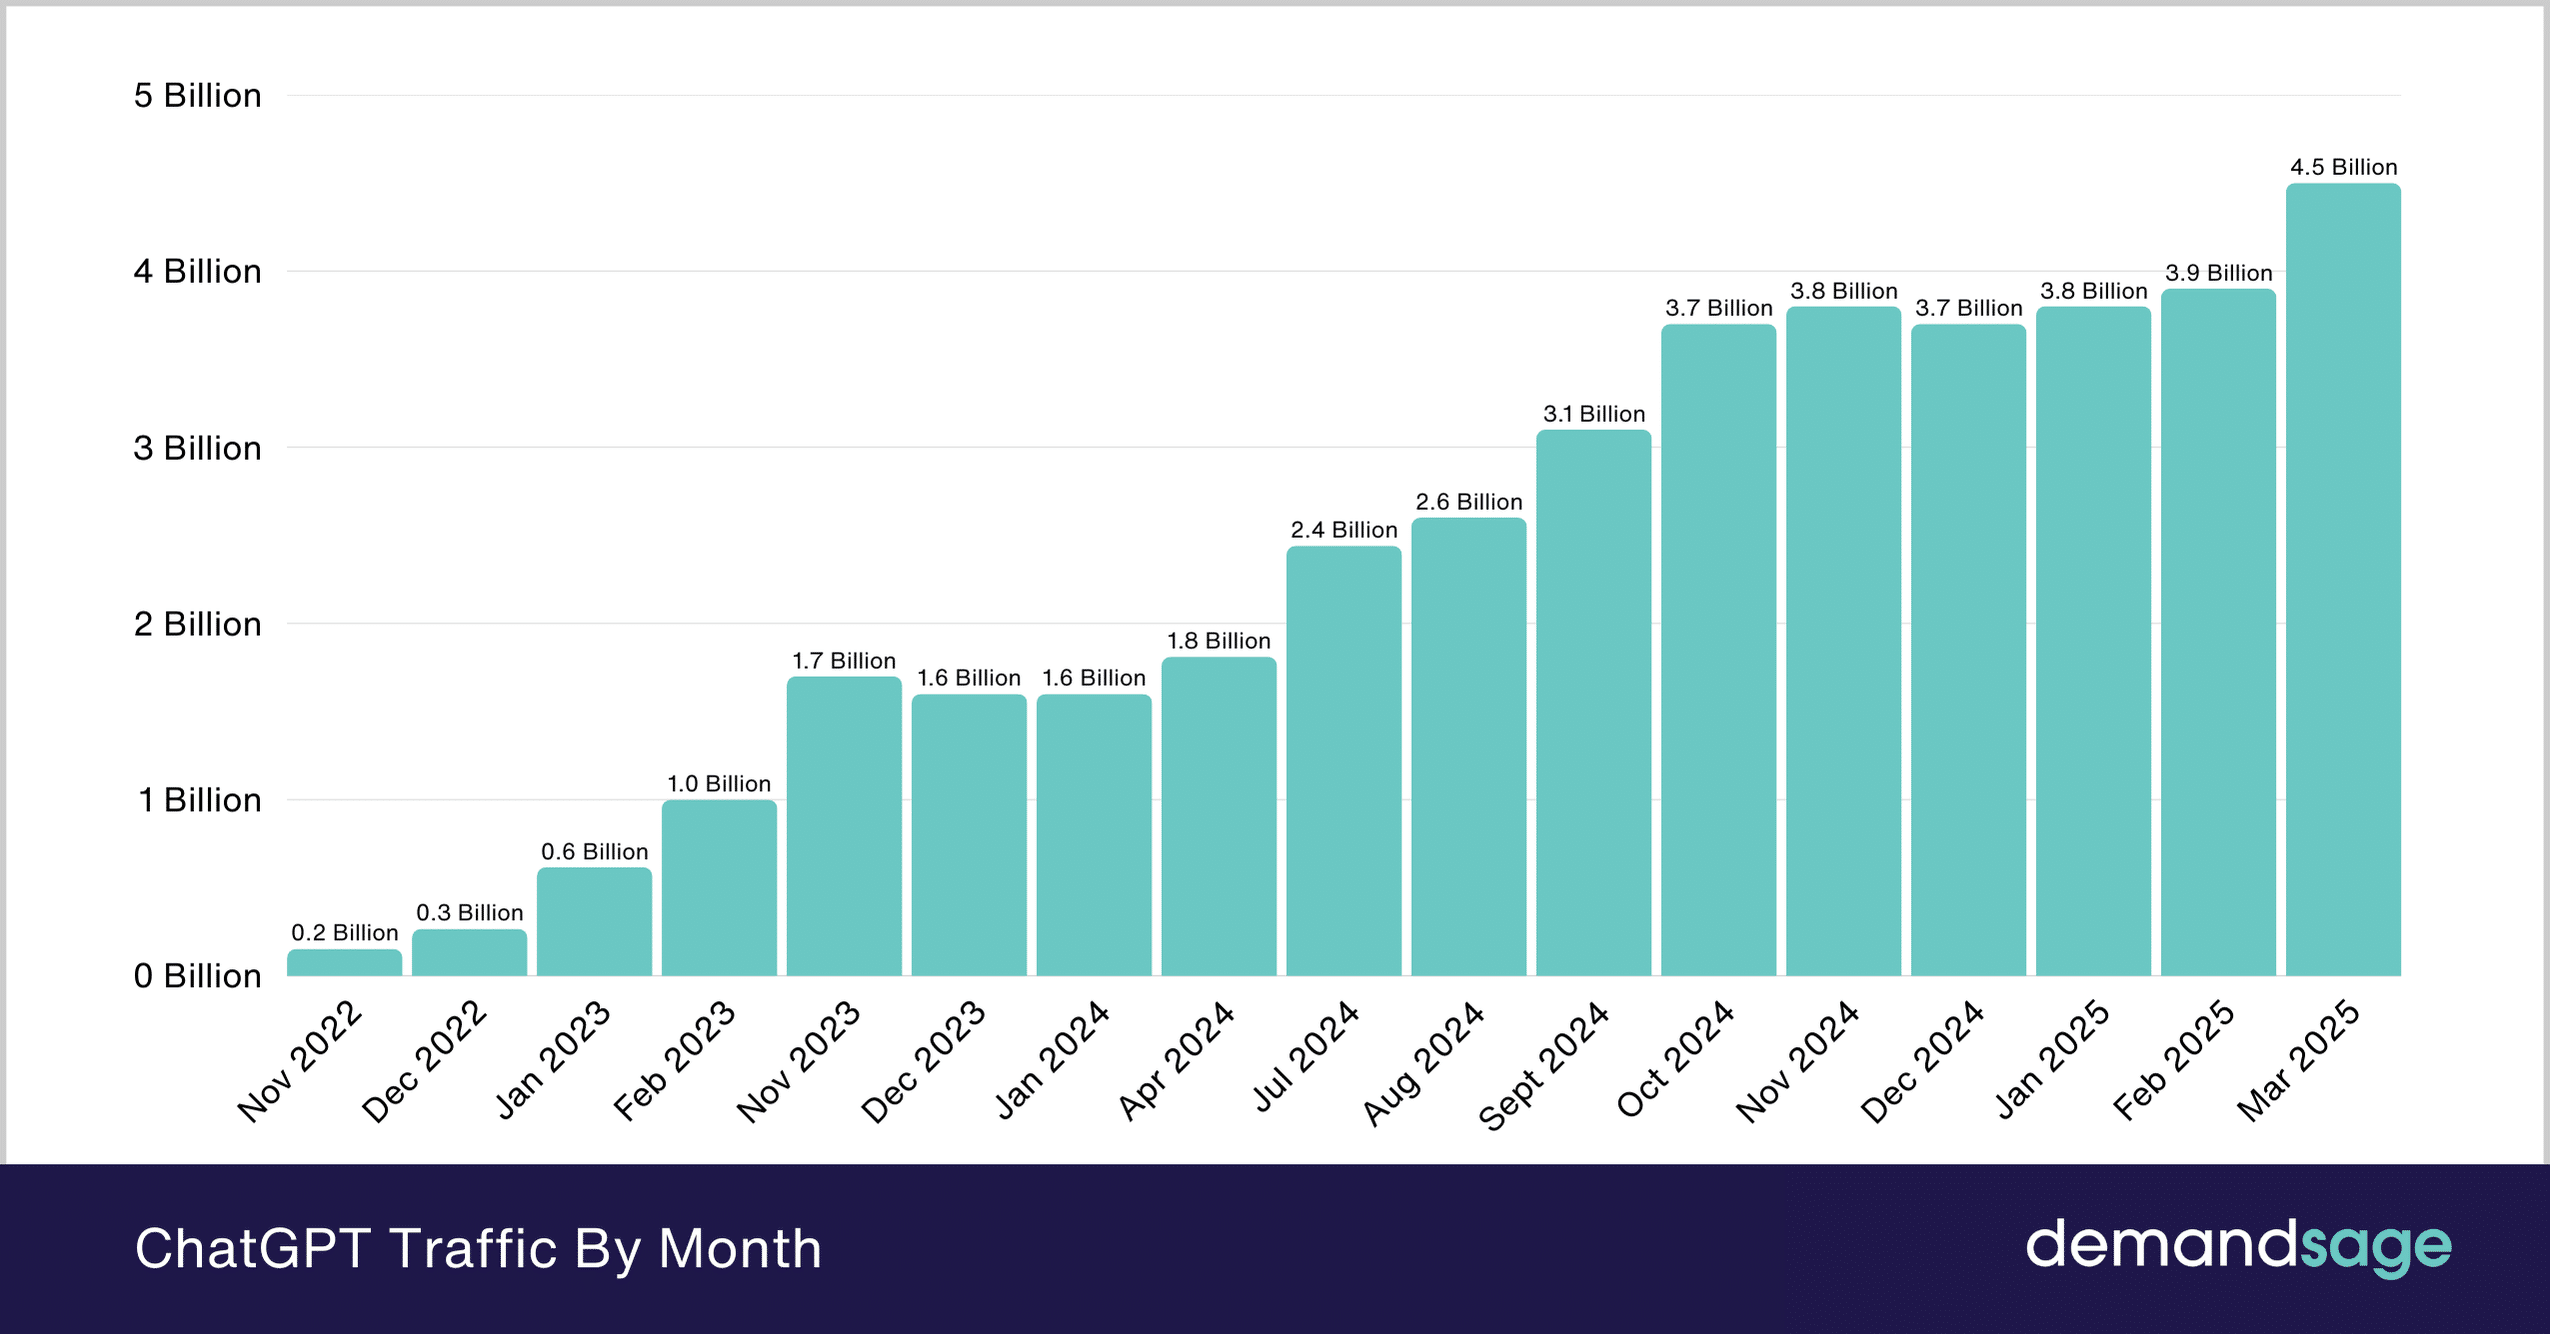
\includegraphics[width=0.75\textwidth]{images/ChatGPTTraffic.png}
    \caption{Evolución del número de consultas diarias (en miles de millones) a ChatGPT \cite{ChatGPTTraffic}.}
    \label{data_evolution}
\end{figure}

Como se observa, la tendencia es claramente ascendente, y la adopción de este tipo de modelos continúa expandiéndose en múltiples sectores. En particular, su uso en el ámbito académico y empresarial se ha vuelto cada vez más común, no solo para generar respuestas simples, sino para realizar tareas complejas como la comprensión y el análisis de documentos extensos.

\vspace{0.3cm}
\textbf{Propósito y objetivos de este trabajo}

Este Trabajo de Fin de Grado aborda un problema concreto: la \textbf{consulta local y privada de documentos técnicos extensos} —en particular, pliegos de contratación pública de entre 30 y 100 páginas— mediante la arquitectura \textit{GraphRAG} (\textit{Retrieval-Augmented Generation} con grafos de conocimiento). El sistema permite formular preguntas en lenguaje natural sobre dichos documentos sin enviar información a servicios externos, combinando recuperación semántica, un grafo de conocimiento jerárquico y agentes de decisión. Sus objetivos principales son:

\begin{itemize}
    \item Desarrollar un módulo de segmentación jerárquica de documentos PDF que preserve la estructura de secciones y subsecciones tal como aparece en el índice original.
    \item Construir un grafo de conocimiento documental que codifique relaciones jerárquicas, secuenciales y semánticas entre los fragmentos de texto.
    \item Implementar agentes de decisión que seleccionen dinámicamente la estrategia de recuperación más adecuada para cada consulta del usuario.
    \item Validar el sistema sobre documentos reales, cuantificando la mejora frente al RAG vectorial tradicional mediante métricas automáticas y un estudio de ablación por componentes.
    \item Demostrar la viabilidad de un despliegue completamente local, sin envío de datos a servidores externos, adecuado para entornos con requisitos de privacidad estrictos.
\end{itemize}

\textbf{Alcance del trabajo.} El sistema se diseña y valida sobre pliegos de prescripciones técnicas y cláusulas administrativas en español, dominio en el que se concentran tanto el diseño del extractor jerárquico como la mayor parte de la evaluación experimental. Se incluye una prueba de generalización sobre documentos de ciberseguridad (véase Capítulo~\ref{cap7}), pero la extensión sistemática a otros dominios documentales queda fuera del alcance de este TFG. Los resultados de la evaluación deben interpretarse como evidencia exploratoria: los tamaños de muestra empleados —entre 8 y 50 preguntas según el experimento— son adecuados para un trabajo de esta naturaleza, pero no permiten establecer conclusiones estadísticamente robustas ni generalizar el rendimiento a cualquier tipo de documento o consulta.

La motivación concreta que originó este trabajo —tanto personal como empresarial— se desarrolla en el Capítulo~\ref{cap3}. Las secciones siguientes establecen el marco teórico necesario para comprender los fundamentos tecnológicos sobre los que se construye la solución.
\newpage
\section{Marco Teórico.}

\subsection{Definición del Problema Central}\label{sec:problema_central}

El problema central que aborda este trabajo puede formularse del siguiente modo: dado un conjunto de documentos técnicos extensos —en concreto, pliegos de prescripciones técnicas y cláusulas administrativas de contratación pública, con un tamaño habitual de entre 30 y 100 páginas—, el objetivo es construir un sistema que permita a un usuario formular preguntas en lenguaje natural y obtener respuestas fundamentadas en el contenido del propio documento, de forma completamente local, sin enviar información a servicios externos.

Este problema presenta tres retos técnicos fundamentales que justifican la arquitectura propuesta:

\begin{enumerate}
    \item \textbf{Limitación de la ventana de contexto:} Los modelos de lenguaje desplegables localmente en hardware de usuario (modelos de 7B--13B parámetros) operan con ventanas de contexto de 8.000--32.000 tokens, muy por debajo de los 60.000 o más tokens que puede contener un documento técnico completo. Enviar el documento íntegro al modelo no es posible en la mayoría de casos.
    \item \textbf{Pérdida de jerarquía documental:} Los sistemas RAG tradicionales dividen el documento en fragmentos independientes, perdiendo las relaciones padre-hijo entre secciones. Una subsección breve (p.ej. ``1.2.3. Requisitos de anclaje'') carece de significado sin el contexto de su sección padre (``1.2. Rack de comunicaciones'').
    \item \textbf{Privacidad y soberanía del dato:} Los pliegos de contratación pública pueden contener información estratégica y comercial sensible que no puede ser procesada en plataformas de nube de terceros sin riesgo legal o de cumplimiento normativo.
\end{enumerate}

La solución propuesta —el sistema \textit{GraphRAG} local— combina la recuperación semántica con un grafo de conocimiento jerárquico y agentes de decisión, abordando simultáneamente los tres retos enumerados. Las secciones siguientes del marco teórico proporcionan los fundamentos conceptuales de cada componente de esta solución: los modelos de lenguaje y sus limitaciones, la arquitectura RAG, los agentes inteligentes y las bases de datos vectoriales.

\subsection{Inteligencia Artificial: Conceptos Generales}
La Inteligencia Artificial puede definirse como el campo de estudio que busca dotar a las máquinas de capacidades cognitivas similares a las del ser humano.
La IA es un campo muy extenso que reúne un conjunto de conceptos que le permiten imitar capacidades intrínsecamente humanas, como el aprendizaje, el reconocimiento de formas, la percepción o la resolución de problemas complejos.
Para llevar a cabo estas tareas se nutre de una amplia variedad de disciplinas, como las matemáticas, la lógica, la informática, e incluso otras como la neurociencia o la lingüística.

\vspace{0.3cm}
\textbf{Clasificación de la IA}

La IA puede clasificarse de distintas formas, siendo las más comunes:

\begin{itemize}
    \item \textbf{Por nivel de capacidad:}
    \begin{itemize}
        \item \textbf{IA débil o estrecha:} Diseñada para realizar tareas específicas (ej. clasificación de imágenes, asistentes por voz(Amazon Alexa)), incluso algunos LLMs como ChatGPT o DeepSeek entran en este nivel, hoy en día es el único tipo de IA que existe.
        \item \textbf{IA general o sólida:} Capaz de realizar cualquier tarea cognitiva humana, esta IA, es capaz de utilizar conocimientos y habilidades previamente aprendidas para la resolución de las mismas, a día de hoy, es simplemente un concepto teórico.
        \item \textbf{Súper IA:} Al igual que la IA general, es meramente una suposición teórica. De hacerse realidad, pensaría, aprendería y razonaría de manera superior a la humana; estas aplicaciones teóricas habrían evolucionado hasta el punto de comprender aspectos humanos como los sentimientos.
    \end{itemize}

    \item \textbf{Por funcionalidades:}
    \begin{itemize}
        \item \textbf{IA mecánica reactiva:} Sistemas que siguen instrucciones explícitas para realizar una tarea específica, sin capacidad de recordar resultados o decisiones anteriores, trabajando únicamente con los datos disponibles en el momento. Esta rama proviene de la matemática estadística y es capaz de analizar grandes cantidades de datos (por ejemplo, el motor de recomendaciones de Netflix usa el historial de visualización para recomendar contenido con mayor probabilidad de ser del agrado del usuario).
        \item \textbf{IA de memoria limitada:} Sistemas que pueden recordar eventos y resultados pasados, permitiendo utilizar estos datos para decidir el curso de acción más probable con el fin de lograr el resultado esperado.
        Estos datos, no se retienen de manera tradicional guardándolos en algún lugar, sino que es entrenada con esos datos, permitiendo mejorar el rendimiento con un mayor número de datos.
        Algunos ejemplos son la IA Generativa (ChatGPT...), vehículos autónomos...
        \item \textbf{IAs con funcionalidades teóricas:} Abarca tanto la teoría de la mente en IA como la IA autoconsciente; ambas son aún teóricas. La primera sería capaz de analizar datos (voces, imágenes, etc.) con el fin de comprender pensamientos y emociones y simular relaciones similares a las humanas, mientras que la IA autoconsciente sería capaz de comprender emociones y pensamientos humanos y desarrollar los propios.
    \end{itemize}
\end{itemize}

A continuación, se presenta una tabla resumen de los principales tipos de IA según distintos criterios de clasificación.

\vspace{0.5cm}
\begin{table}[H]
\centering
\caption{Clasificación de la Inteligencia Artificial}
\begin{tabular}{|p{3.5cm}|p{4.5cm}|p{6cm}|}
\hline
\textbf{Criterio} & \textbf{Tipo de IA} & \textbf{Descripción y ejemplos} \\
\hline
\multirow{3}{*}{\textbf{Por capacidad}} 
& IA débil & Especializada en tareas concretas. Ej: Alexa, Siri, ChatGPT. \\
& IA general & Teórica. Capaz de realizar cualquier tarea cognitiva humana. \\
& Súper IA & Hipotética. Superaría al ser humano en inteligencia y emociones. \\
\hline
\multirow{3}{*}{\textbf{Por funcionalidad}} 
& Mecánica reactiva & No guarda memoria. Reacciona en tiempo real. Ej: Recomendaciones de Netflix. \\
& Memoria limitada & Aprende de datos previos. Ej: ChatGPT, vehículos autónomos. \\
& IA teórica & Incluye teoría de la mente y autoconsciencia. Aún no desarrolladas. \\
\hline
\end{tabular}
\label{tab:clasificacion_ia}
\end{table}


\newpage
\textbf{Machine Learning (ML)}

El \textit{Machine Learning} es una rama de la IA que se centra en el entrenamiento de las máquinas con el fin de imitar el aprendizaje humano, siendo así capaces de realizar tareas de forma autónoma y de mejorar su rendimiento mediante una mayor exposición a datos y la propia experiencia con los mismos.
De acuerdo con \cite{ibmML2024}, un sistema de aprendizaje automático puede describirse a través de tres componentes fundamentales:

    \begin{itemize}
        \item \textbf{El proceso de decisión:} Generalmente los algoritmos de Machine Learning son utilizados para realizar predicciones o clasificaciones en base a unos datos de entrada (etiquetados o no) de los cuales el algoritmo hará una estimación.
        \item \textbf{Función de error:} Es aquella función que 
        compara los resultados con ejemplos conocidos para evaluar el desempeño del algoritmo.
        \item \textbf{Optimización del modelo:} Un método mediante el cual el algoritmo evalúa los fallos y actualiza el proceso de decisión (Principalmente mediante pesos), este procedimiento generalmente es repetido de manera iterativa.
    \end{itemize}

A continuación, sin entrar en profundidad en las implementaciones, se describen los principales tipos de aprendizaje automático:

\begin{itemize}
    \item \textbf{Aprendizaje supervisado:} Se utilizan datos etiquetados para el entrenamiento, con el fin de clasificar o predecir resultados; los pesos del modelo se ajustan a medida que se introducen datos. (Ejemplos: Regresión Lineal, Random Forest y Máquinas de Soporte Vectorial (SVM).)
    \item \textbf{Aprendizaje no supervisado:} Se emplean algoritmos de \textit{Machine Learning} para clasificar conjuntos de datos sin etiquetar, es decir, sin necesidad de intervención humana directa para las agrupaciones. (Ejemplos: Clustering, Reducción de Dimensionalidad y \textit{Autoencoders}.)
    \item \textbf{Aprendizaje semisupervisado:} Punto intermedio entre los dos tipos anteriores; combina un pequeño conjunto de datos etiquetados con uno mayor sin etiquetar, lo que permite paliar el problema de la escasez de datos etiquetados.
    \item \textbf{Aprendizaje por refuerzo:} En cierto modo similar al aprendizaje supervisado, pero en lugar de utilizar datos de muestra, el modelo aprende mediante prueba y error, reforzando la secuencia de acciones que produce resultados más exitosos.
\end{itemize}

\vspace{0.5cm}
\begin{table}[H]
\centering
\caption{Resumen Tipos de aprendizaje en Machine Learning}
\begin{tabular}{|p{3.5cm}|p{6cm}|p{4.5cm}|}
\hline
\textbf{Tipo de aprendizaje} & \textbf{Descripción} & \textbf{Ejemplos comunes} \\
\hline
\textbf{Supervisado} & Utiliza datos etiquetados. El algoritmo aprende una función a partir de pares entrada-salida. & Regresión lineal, Random Forest, SVM. \\
\hline
\textbf{No supervisado} & Usa datos sin etiquetar. El modelo identifica patrones o estructuras ocultas. & Clustering, PCA, Autoencoders. \\
\hline
\textbf{Semisupervisado} & Combina un pequeño conjunto etiquetado con una gran cantidad sin etiquetar. Reduce necesidad de anotaciones humanas. & Clasificadores combinados con técnicas de propagación de etiquetas. \\
\hline
\textbf{Por refuerzo} & Aprende mediante prueba y error. Recibe recompensas o penalizaciones según su rendimiento. & Robots autónomos, sistemas de control de videojuegos. \\
\hline
\end{tabular}
\label{tab:tipos_aprendizaje}
\end{table}


\newpage
\textbf{Diferencias entre Deep Learning (DL), Machine Learning (ML) y Neural Networks (NN)}

Con frecuencia, estos términos se utilizan de manera indistinta; a continuación se presenta una diferenciación precisa de cada uno antes de profundizar en los LLMs.

El \textbf{Deep Learning (DL)} es un subcampo dentro de las \textbf{Redes Neuronales Artificiales (NN)}, las cuales, a su vez, son un subcampo del \textbf{Machine Learning (ML)}. Esta relación puede visualizarse como una jerarquía en la que la Inteligencia Artificial engloba al Machine Learning, este a las Redes Neuronales, y estas últimas al Deep Learning.

\begin{itemize}
    \item \textbf{Machine Learning (ML):} Se refiere a sistemas capaces de aprender de los datos mediante algoritmos estadísticos y mejorar su rendimiento con la experiencia. Puede incluir métodos como árboles de decisión, regresión logística, máquinas de soporte vectorial, y también redes neuronales básicas. Requiere habitualmente intervención humana para la selección de características y para estructurar los datos de entrada.
    
    \item \textbf{Neural Networks (NN):} Son modelos inspirados en el funcionamiento del cerebro humano y forman parte de los algoritmos de ML. Consisten en capas de nodos o neuronas artificiales conectadas entre sí, que permiten realizar tareas complejas de clasificación y regresión. Una red neuronal simple consta de una capa de entrada, una o más capas ocultas, y una capa de salida.
    
    \item \textbf{Deep Learning (DL):} Es un tipo de red neuronal con múltiples capas ocultas (generalmente más de tres), lo que le otorga mayor capacidad de abstracción y permite trabajar con grandes volúmenes de datos no estructurados como imágenes, texto o audio. A diferencia del ML tradicional, el DL automatiza la extracción de características, lo que reduce la necesidad de intervención humana y permite abordar tareas más complejas como el reconocimiento de voz, visión por computadora o procesamiento del lenguaje natural.
\end{itemize}

En resumen, mientras que el Machine Learning incluye una gran variedad de técnicas de aprendizaje automático, las redes neuronales constituyen una familia de modelos dentro de ese conjunto, y el Deep Learning se distingue por su profundidad y capacidad para manejar datos no estructurados y problemas de alta complejidad. Esta base técnica resulta fundamental para comprender cómo operan los Modelos de Lenguaje de Gran Escala (LLMs), cuya arquitectura se basa en redes neuronales profundas, especialmente del tipo \textit{Transformer}.

\newpage
\subsection{Historia y Evolución}
No todos estos términos aparecieron de forma simultánea; se fueron produciendo avances paulatinos hasta conformar lo que es hoy la IA. A continuación se presenta un breve resumen de su historia.

\vspace{0.3cm}
\textbf{Alan Turing y los inicios de la IA (décadas de 1940 y 1950)}

Alan Turing es considerado como el pionero de la IA, fue un lógico y matemático que hizo los avances iniciales en el campo. En 1950 propuso el test de Turing, una prueba para evaluar la inteligencia de una máquina, en el artículo \textit{Computing Machinery and Intelligence} \cite{Turing1950}, en el cual planteaba la pregunta: \textit{Can machines think?}, es decir, ¿Pueden las máquinas pensar?.\\
\\
En esta época se sientan las bases teóricas, con la aparición de algoritmos simbólicos que intentan emular el razonamiento humano mediante reglas explícitas obtenidas mediante la lógica formal.

\vspace{0.3cm}
\textbf{Nacimiento formal y primer auge (1956–1970)}

En 1956, se celebra la conferencia de Dartmouth, organizada por John McCarthy, Marvin Minsky, Nathaniel Rochester y Claude Shannon. Este evento es considerado el nacimiento oficial de la IA como disciplina académica. Durante este período, se desarrollaron los primeros programas de IA capaces de resolver problemas matemáticos, jugar al ajedrez o simular conversaciones, como ELIZA (1966).

El optimismo de esta etapa llevó a pensar que pronto se alcanzaría una inteligencia similar a la humana. Sin embargo, las limitaciones tecnológicas y la falta de datos reales demostraron que la IA simbólica tenía dificultades para escalar a problemas más complejos o con alta variabilidad.

\vspace{0.3cm}
\textbf{Estancamiento y \textit{invierno de la IA} (1970–1980)}

A partir de los años 70, las expectativas no cumplidas y los escasos resultados prácticos provocaron una pérdida de interés y financiación en el campo. Este periodo, conocido como el \textit{invierno de la IA}, se caracterizó por el estancamiento de la investigación y una visión más crítica del potencial de la inteligencia artificial. Muchos de los problemas de la IA no venían dados únicamente por limitaciones lógicas, sino también por las restricciones del propio hardware, circunstancia que, en menor escala, también se ha podido constatar durante el desarrollo de este proyecto.

\vspace{0.3cm}
\textbf{Renacimiento: Machine Learning y redes neuronales (1990–2000)}

Durante las décadas de 1980 y 1990 (con mayor incidencia en la segunda), la IA comenzó a orientarse hacia enfoques más estadísticos y empíricos. Nace así el \textit{Machine Learning}, que abandona en parte las reglas explícitas y se basa en la capacidad de los algoritmos para aprender a partir de datos. Se retoman también las redes neuronales artificiales, aunque de manera limitada, debido a restricciones computacionales.

En paralelo, el aumento de la potencia de cálculo y la disponibilidad de grandes volúmenes de datos comenzaron a marcar una nueva etapa para la IA, más centrada en aplicaciones prácticas como el reconocimiento óptico de caracteres o los sistemas expertos, los cuales destacarían en esta etapa concreta.

\vspace{0.3cm}
\textbf{Explosión del Deep Learning y la IA moderna (2010–actualidad)}

A partir de 2012, se produce un cambio radical con la victoria de \textit{AlexNet} en el concurso de visión por computadora ImageNet, marcando el inicio del auge del \textit{Deep Learning}. Este enfoque, basado en redes neuronales profundas, permite resolver tareas complejas como reconocimiento facial, traducción automática o conducción autónoma con una precisión sin precedentes.

En 2017, Google presenta la arquitectura \textit{Transformer}, que revoluciona el campo del procesamiento del lenguaje natural (NLP) al permitir un entrenamiento más eficiente y eficaz de modelos sobre grandes cantidades de texto. Esto da lugar al desarrollo de los primeros Modelos de Lenguaje de Gran Escala (LLMs), como BERT (2018), GPT-2 (2019), GPT-3 (2020) y sus sucesores, que constituyen el eje central de este trabajo y se analizan con mayor detalle en la subsección correspondiente.

\vspace{0.3cm}
\textbf{Conclusión}

La historia de la Inteligencia Artificial está marcada por ciclos de entusiasmo y escepticismo, pero su desarrollo ha sido continuo y progresivo. Comprender esta evolución resulta fundamental para contextualizar el surgimiento de los LLMs y valorar el impacto que tienen hoy en día en múltiples sectores. Desde las ideas teóricas de Turing hasta los modelos generativos modernos, la IA ha recorrido un largo camino que continúa redefiniendo nuestra relación con la tecnología, y, en el momento de redactar este trabajo, la IA se encuentra en un período de auge sostenido. Si bien la IA generativa genera debate académico sobre la sostenibilidad de este crecimiento, la combinación de avances en hardware, la disponibilidad de datos y la inversión industrial sin precedentes sugiere un contexto estructuralmente diferente al que precedió al estancamiento de la década de 1970.

Establecida esta base histórica, la siguiente subsección se centra en el componente más relevante para este proyecto: los LLMs.
\newpage

\subsection{Modelos de Lenguaje de Gran Escala (LLMs)}

\textbf{Definición y características generales} \\
Los Modelos de Lenguaje de Gran Escala (\textit{Large Language Models}, LLMs) son modelos de aprendizaje profundo basados principalmente en la arquitectura \textbf{Transformer} \cite{Vaswani2017}, entrenados con corpus masivos para aproximar distribuciones de probabilidad sobre secuencias de tokens.  

En su forma autoregresiva, un LLM modela:
\[
p(x_t \mid x_{<t}) 
\]
y aprende a predecir el \textit{próximo token} dado un contexto; en su forma enmascarada (\textit{masked}), optimiza la recuperación de tokens ocultos dentro de la secuencia \cite{Devlin2018}. Esta formulación permite realizar tareas de comprensión y generación de lenguaje natural con alta coherencia y cobertura.

A nivel práctico, los LLMs operan sobre \textbf{subpalabras} (\textit{subword units}) obtenidas mediante técnicas de tokenización como BPE o SentencePiece \cite{Sennrich2016,Kudo2018}, e incorporan información posicional (codificación absoluta o relativa) para mantener el orden secuencial.  

Su \textbf{escala} —tanto en parámetros como en datos— es determinante: al aumentar tamaño y cómputo, los modelos exhiben leyes de escalado \cite{Kaplan2020} y, con una asignación de datos-cómputo eficiente, alcanzan óptimos de entrenamiento (\textit{compute-optimal}) \cite{Hoffmann2022}.

\vspace{0.3cm}
\textbf{De NLP clásico a LLMs} \\
La evolución hacia los LLMs procede de:
\begin{enumerate}
    \item Sistemas basados en reglas.
    \item Modelos estadísticos (\textit{n-gramas}).
    \item Representaciones distribuidas (Word2Vec, GloVe).
    \item Redes recurrentes (RNN/LSTM/GRU), limitadas para dependencias largas.
    \item \textbf{Transformers}, que mediante \textit{self-attention} procesan la secuencia en paralelo y capturan dependencias a largo alcance \cite{Vaswani2017}.
\end{enumerate}

Sobre esta base se construyen familias como BERT (preentrenamiento \textit{masked}) \cite{Devlin2018} y GPT (autoregresivo) \cite{Brown2020}.

\begin{table}[H]
\centering
\begin{tabular}{|p{3cm}|p{4cm}|p{4cm}|}
\hline
\textbf{Etapa} & \textbf{Modelo / Técnica} & \textbf{Limitación / Avance} \\
\hline
Basado en reglas & Gramáticas formales, ELIZA & No generalizan, rigidez ante variación lingüística \\
\hline
Estadístico & N-gramas, Markov & Incapacidad para dependencias largas \\
\hline
Embeddings & Word2Vec, GloVe & Semántica distribuida, sin contexto dinámico \\
\hline
Secuenciales & RNN, LSTM, GRU & Gradientes/escape a largo plazo, poca paralelización \\
\hline
Transformers & BERT, GPT, LLMs & Atención paralelizable, dependencias largas y escalado \\
\hline
\end{tabular}
\caption{Evolución resumida del PLN hacia LLMs.}
\end{table}

\vspace{0.3cm}
\textbf{Capacidades y propiedades de los LLMs} 
\begin{itemize}
    \item \textbf{Aprendizaje en contexto} (\textit{in-context learning}): seguir instrucciones y realizar tareas nuevas a partir de pocos ejemplos, sin actualizar parámetros \cite{Brown2020}.
    \item \textbf{Generalización de tareas}: clasificación, extracción de información, QA, resumen, traducción, razonamiento y generación de código.
    \item \textbf{Escalado y capacidades emergentes}: mejora sistemática con más datos, parámetros y cómputo \cite{Kaplan2020,Hoffmann2022}.
    \item \textbf{Multimodalidad}: incorporación de visión y audio en un mismo modelo (p.ej., variantes GPT-4V) \cite{OpenAI2023}.
\end{itemize}

\vspace{0.3cm}
\textbf{Ciclo de entrenamiento y alineación} 
\begin{enumerate}
    \item \textbf{Preentrenamiento} autosupervisado (objetivo causal o enmascarado) sobre corpus heterogéneos.
    \item \textbf{Ajuste fino supervisado} (\textit{SFT}) con pares pregunta–respuesta.
    \item \textbf{Alineación con preferencias humanas}: \textit{Reinforcement Learning from Human Feedback} (RLHF), donde un modelo de recompensa aprendido a partir de comparaciones humanas guía la política del LLM \cite{Ouyang2022}.
\end{enumerate}

Para despliegues eficientes se emplean \textbf{adaptadores y entrenamiento eficiente} (LoRA/QLoRA) que ajustan un subconjunto de parámetros, reduciendo memoria y coste \cite{Hu2021,Dettmers2023}.

\vspace{0.3cm}
\textbf{Evaluación} 
\begin{itemize}
    \item \textbf{Perplejidad}: calidad del modelado del lenguaje.
    \item \textbf{Baterías de tareas}: MMLU \cite{Hendrycks2021}, BIG-bench \cite{Srivastava2022}, evaluaciones de diálogo/código (MT-Bench, HumanEval).
    \item \textbf{Evaluación holística}: HELM \cite{Liang2022}, integrando calidad, robustez y riesgos (\textit{harms}).
\end{itemize}

\vspace{0.3cm}
\textbf{Limitaciones y retos abiertos} 
\begin{itemize}
    \item \textbf{Contexto limitado y costes}: atención cuadrática; investigación en atención eficiente y contextos extendidos.
    \item \textbf{Alucinaciones y veracidad}: generación plausible pero falsa; mitigación con datos, calibración y RAG.
    \item \textbf{Sesgos y seguridad}: reflejo de sesgos del corpus, contenido dañino o ataques de \textit{prompt injection}.
    \item \textbf{Interpretabilidad}: difícil atribuir razonamientos en modelos grandes.
    \item \textbf{Eficiencia y sostenibilidad}: alta demanda de energía y hardware; mitigación con cuantización, destilación o \textit{mixture-of-experts}.
\end{itemize}

\vspace{0.3cm}
\textbf{Panorama actual y tendencias} 
\begin{itemize}
    \item Modelos abiertos eficientes (LLaMA, Mistral) \cite{Touvron2023}.
    \item Adaptaciones ligeras para empresas (LoRA/QLoRA).
    \item Multimodalidad y uso de herramientas (\textit{tool-use}/APIs).
    \item Integración con recuperación externa (RAG) para actualización factual y trazabilidad.
\end{itemize}


\newpage
\subsection{Limitaciones de los LLMs: El Problema del Contexto}

Aunque los LLMs han demostrado una capacidad extraordinaria para el procesamiento del lenguaje, presentan una limitación estructural que condiciona directamente su aplicabilidad en entornos empresariales con documentación extensa: la \textbf{ventana de contexto}.

\vspace{0.3cm}
\textbf{La ventana de contexto}

La arquitectura Transformer procesa la entrada como una secuencia de \textit{tokens}. El mecanismo de \textit{self-attention} calcula relaciones entre todos los pares de tokens de la secuencia, lo que implica una complejidad computacional de orden $\mathcal{O}(n^2)$ en memoria y cómputo, siendo $n$ la longitud de la secuencia. Esta dependencia cuadrática hace que ampliar la ventana de contexto sea costoso tanto en tiempo como en memoria de GPU.

En la práctica, los modelos más accesibles operan con ventanas de entre 4.096 y 32.768 tokens, mientras que los modelos con contextos extendidos (128K--1M tokens) requieren hardware de alto coste y exhiben tiempos de inferencia significativamente mayores. A modo de referencia, un documento técnico de 100 páginas puede superar los 60.000 tokens, muy por encima del límite de la mayoría de modelos desplegables localmente.

\vspace{0.3cm}
\textbf{Degradación de la calidad: \textit{Lost in the Middle}}

Incluso cuando la longitud del documento se sitúa dentro de la ventana permitida, la calidad de las respuestas no es uniforme. La investigación de \cite{liu2024lost} demuestra empíricamente que los modelos de lenguaje tienden a recordar mejor la información situada al principio y al final del contexto, mientras que el contenido en posiciones intermedias es frecuentemente ignorado o mal interpretado. Este fenómeno, denominado \textit{Lost in the Middle}, implica que \textbf{aumentar el contexto no equivale a mejorar la comprensión}.

\vspace{0.3cm}
\textbf{Alucinaciones por falta de información}

Cuando el modelo no dispone de información suficiente en su contexto para responder una pregunta, no siempre reconoce su propia ignorancia: en lugar de responder ``no lo sé'', puede generar una respuesta plausible pero falsa, fenómeno conocido como \textbf{alucinación}. En entornos empresariales donde se trabaja con documentos jurídicos o técnicos, este comportamiento supone un riesgo inaceptable.

\vspace{0.3cm}
\textbf{Implicaciones para este proyecto}

Las limitaciones descritas justifican la necesidad de un enfoque alternativo al simple volcado de documentos completos en el contexto del modelo. En concreto, este proyecto aborda el problema mediante dos estrategias complementarias:

\begin{itemize}
    \item \textbf{Recuperación selectiva de contexto (RAG):} en lugar de enviar el documento íntegro, se identifican y entregan al modelo únicamente los fragmentos más relevantes para cada consulta.
    \item \textbf{Agente de selección de estrategia:} un componente inteligente decide dinámicamente si es posible operar con fragmentos o si la consulta exige el documento completo, gestionando así el presupuesto de tokens de forma eficiente.
\end{itemize}

\newpage
\subsection{Retrieval-Augmented Generation (RAG)}

El \textbf{Retrieval-Augmented Generation} (RAG) es una arquitectura que combina la capacidad generativa de los LLMs con un sistema externo de recuperación de información \cite{Lewis2020}. El objetivo es proporcionar al modelo el contexto relevante en el momento de la inferencia, sin necesidad de reentrenar el modelo ni ampliar artificialmente su ventana de contexto.

\vspace{0.3cm}
\textbf{Pipeline clásico de RAG}

Un sistema RAG convencional sigue las siguientes etapas \cite{Gao2023}:

\begin{enumerate}
    \item \textbf{Ingesta y chunking:} los documentos se dividen en fragmentos (\textit{chunks}) de tamaño manejable. La estrategia de segmentación influye directamente en la calidad de la recuperación: fragmentos demasiado pequeños pierden contexto; demasiado grandes saturan la ventana del modelo.
    \item \textbf{Generación de embeddings:} cada fragmento se transforma en un vector numérico de alta dimensión mediante un modelo de codificación semántica (\textit{embedding model}), de forma que fragmentos con contenido similar queden próximos en el espacio vectorial.
    \item \textbf{Almacenamiento en índice vectorial:} los vectores se indexan en una estructura que permite realizar búsquedas eficientes por similitud (ANN, \textit{Approximate Nearest Neighbor}).
    \item \textbf{Recuperación:} ante una consulta del usuario, esta se codifica con el mismo modelo de embeddings y se recuperan los fragmentos más similares del índice.
    \item \textbf{Generación aumentada:} los fragmentos recuperados se incluyen en el \textit{prompt} del LLM junto con la consulta original, permitiendo al modelo generar una respuesta fundamentada en el contenido real del documento.
\end{enumerate}

\begin{figure}[H]
    \centering
    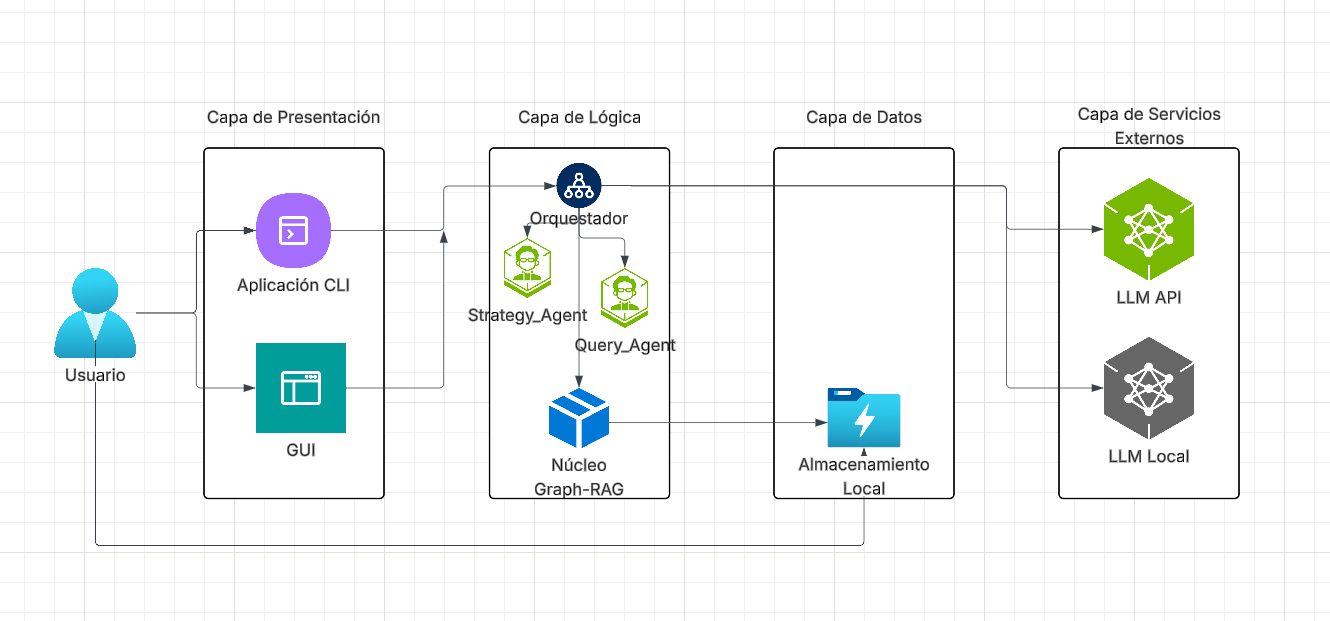
\includegraphics[width=0.9\textwidth]{images/Diagrama_Arquitectura.png}
    \caption{Diagrama de arquitectura del sistema GraphRAG desarrollado en este proyecto.}
    \label{fig:arq_intro}
\end{figure}

\vspace{0.3cm}
\textbf{Estrategias de chunking}

La forma en que se divide el documento determina la granularidad del conocimiento recuperable. Las estrategias más habituales son:

\begin{itemize}
    \item \textbf{Chunking fijo:} división por número de caracteres o tokens. Sencillo de implementar pero ignora la estructura semántica del texto, generando cortes en mitad de ideas o secciones.
    \item \textbf{Chunking con solapamiento (\textit{sliding window}):} introduce un solapamiento entre fragmentos consecutivos para preservar el contexto en los límites. Mejora la recuperación de frases cercanas a los bordes de los chunks.
    \item \textbf{Chunking jerárquico o estructural:} aprovecha la estructura del documento (índice, secciones, subsecciones) para definir las fronteras de cada fragmento. Preserva la integridad semántica de cada sección y permite reconstruir relaciones padre-hijo entre fragmentos. \textbf{Esta es la estrategia adoptada en el presente proyecto}, implementada en el módulo \texttt{chunk\_extractor.py}.
\end{itemize}

\vspace{0.3cm}
\textbf{Búsqueda híbrida: semántica y léxica}

La recuperación basada únicamente en similitud vectorial puede fallar ante términos técnicos concretos (códigos, siglas, nombres propios), ya que el embedding los ``diluye'' en el espacio semántico. Para compensarlo, este proyecto implementa una \textbf{búsqueda híbrida} que combina:

\begin{itemize}
    \item \textbf{Similitud de coseno sobre embeddings} (modelo \texttt{all-MiniLM-L6-v2} \cite{Reimers2019}): captura la intención semántica de la consulta.
    \item \textbf{BM25} (\textit{Best Matching 25}) \cite{Robertson2009}: algoritmo probabilístico de recuperación léxica que puntúa documentos en función de la frecuencia e inversión de los términos de la consulta (\textit{TF-IDF} extendido). Detecta con alta precisión términos exactos ausentes en el espacio semántico.
\end{itemize}

\vspace{0.3cm}
\textbf{Limitaciones del RAG clásico y motivación del GraphRAG}

El RAG vectorial tradicional trata cada fragmento de forma aislada, sin tener en cuenta su posición en la estructura del documento. Esto genera dos problemas recurrentes al trabajar con documentos técnicos complejos:

\begin{itemize}
    \item \textbf{Pérdida de jerarquía:} un fragmento de nivel bajo (p.ej. ``\textit{1.2.3. Requisitos de protección física}'') puede ser recuperado sin incluir el contexto de su sección padre (``\textit{1.2. Rack de comunicaciones}''), generando respuestas incompletas.
    \item \textbf{Desconexión entre secciones relacionadas:} dos secciones semánticamente relacionadas pero ubicadas en distintos capítulos no están conectadas en un sistema RAG clásico.
\end{itemize}

La solución adoptada en este proyecto, el \textbf{GraphRAG} \cite{Edge2024}, representa los fragmentos como nodos de un grafo dirigido donde las aristas codifican relaciones jerárquicas, secuenciales y semánticas entre secciones. Esto permite recuperar no solo el fragmento más relevante, sino también su contexto estructural completo, como se detalla en los capítulos de diseño e implementación.

\newpage
\subsection{Agentes y Rerankers}

\textbf{Agentes basados en LLM}

Un \textbf{agente} es un sistema que utiliza un LLM como motor de razonamiento para tomar decisiones y ejecutar acciones de forma autónoma, en función de un objetivo y del estado del entorno \cite{Yao2023}. A diferencia de una llamada directa al modelo, un agente sigue un ciclo iterativo:

\begin{enumerate}
    \item \textbf{Observación:} recibe información del entorno (consulta del usuario, metadatos del documento, resultados de búsquedas anteriores).
    \item \textbf{Razonamiento:} el LLM analiza la observación y decide la acción más adecuada.
    \item \textbf{Acción:} ejecuta la acción seleccionada (llamar a una herramienta, realizar una búsqueda, generar una respuesta).
    \item \textbf{Actualización:} el resultado de la acción se incorpora al contexto para la siguiente iteración.
\end{enumerate}

Este paradigma, popularizado por el framework \textit{ReAct} \cite{Yao2023} (Reasoning + Acting), permite construir sistemas capaces de razonar sobre cuándo y cómo utilizar herramientas externas. En el presente proyecto se implementan dos agentes especializados:

\begin{itemize}
    \item \textbf{Agente de Selección de Estrategia (\texttt{DocumentStrategyAgent}):} analiza la consulta y decide si responder con recuperación selectiva de fragmentos (\texttt{PARTIAL}) o con el documento completo (\texttt{FULL}). Esta decisión condiciona todo el flujo posterior y permite optimizar el consumo de la ventana de contexto.

    \item \textbf{Agente de Optimización de Consulta:} transforma la pregunta original del usuario, que puede contener ruido lingüístico o instrucciones de formato, en una consulta depurada centrada en los términos clave. Esto mejora la precisión de la búsqueda vectorial y léxica.
\end{itemize}

\vspace{0.3cm}
\textbf{Rerankers: bi-encoders vs cross-encoders}

En sistemas RAG, la recuperación inicial devuelve un conjunto de candidatos ordenados por similitud. Sin embargo, los modelos de embedding (\textit{bi-encoders}) calculan los vectores de consulta y documento de forma independiente, lo que introduce un margen de error en el ranking. Para refinarlo, se emplea un \textbf{reranker} basado en \textit{Cross-Encoder} \cite{Reimers2019}.

La diferencia fundamental entre ambos enfoques se resume en la siguiente tabla:

\begin{table}[H]
\centering
\renewcommand{\arraystretch}{1.4}
\caption{Comparativa entre Bi-Encoder y Cross-Encoder.}
\label{tab:biencoder_crossencoder}
\begin{tabularx}{\textwidth}{|l|X|X|}
\hline
\textbf{Característica} & \textbf{Bi-Encoder} & \textbf{Cross-Encoder} \\
\hline
\textbf{Procesamiento} & Consulta y documento codificados por separado & Consulta y documento procesados conjuntamente \\
\hline
\textbf{Velocidad} & Muy rápido (búsqueda por ANN) & Lento (requiere una pasada por par) \\
\hline
\textbf{Precisión} & Aproximada & Alta (analiza interacción directa entre términos) \\
\hline
\textbf{Uso típico} & Recuperación inicial sobre corpus grande & Reordenación (\textit{reranking}) de candidatos \\
\hline
\textbf{Modelo en este proyecto} & \texttt{all-MiniLM-L6-v2} & \nolinkurl{cross-encoder/ms-marco-MiniLM-L-6-v2} \\
\hline
\end{tabularx}
\end{table}

El flujo implementado combina ambos enfoques en dos etapas: primero, el \textit{bi-encoder} recupera eficientemente los candidatos más prometedores del grafo; después, el \textit{Cross-Encoder} reordena esos candidatos evaluando cada par (consulta, fragmento) de forma conjunta, eliminando falsos positivos semánticos y elevando al primer puesto los fragmentos que realmente responden a la pregunta.

\newpage
\subsection{Bases de Datos Vectoriales y LangGraph}

\textbf{Bases de datos vectoriales}

Una \textbf{base de datos vectorial} es un sistema de almacenamiento optimizado para indexar y consultar vectores de alta dimensión mediante búsquedas por similitud aproximada (ANN). A diferencia de las bases de datos relacionales, que buscan coincidencias exactas, las bases vectoriales permiten recuperar los elementos más próximos a un vector de consulta en el espacio de embeddings.

Las soluciones más utilizadas en el ecosistema RAG son:

\begin{table}[H]
\centering
\renewcommand{\arraystretch}{1.4}
\caption{Comparativa de bases de datos vectoriales.}
\label{tab:vectordb_intro}
\begin{tabularx}{\textwidth}{|l|X|l|}
\hline
\textbf{Solución} & \textbf{Características principales} & \textbf{Tipo} \\
\hline
FAISS & Optimizado para GPU, búsqueda en memoria, sin persistencia nativa & Open source \\
\hline
ChromaDB & Sencillo de integrar con LangChain, persistencia local & Open source \\
\hline
Pinecone & SaaS, escalabilidad gestionada, filtros por metadatos & Pago por uso \\
\hline
Weaviate & Orientado a producción, soporte multimodal & Open source / SaaS \\
\hline
\end{tabularx}
\end{table}

En el presente proyecto, dado que los documentos se procesan por sesión sin necesidad de persistencia entre ejecuciones, \textbf{no se utiliza una base de datos vectorial dedicada}. En su lugar, los embeddings se almacenan en memoria como atributos de los nodos del grafo de \texttt{NetworkX}, lo que permite integrar la búsqueda semántica directamente con el análisis estructural del documento. La incorporación de persistencia mediante ChromaDB o FAISS se propone como mejora futura en el capítulo de conclusiones.

\vspace{0.3cm}
\textbf{Grafos de conocimiento con NetworkX}

\texttt{NetworkX} es una librería de Python para la creación, manipulación y análisis de grafos y redes complejas. En este proyecto se utiliza para construir un \textbf{grafo de conocimiento dirigido} (\texttt{DiGraph}) donde:

\begin{itemize}
    \item Cada \textbf{nodo} representa una sección del documento (un \textit{chunk} jerárquico) y almacena su texto, nivel de profundidad, rango de páginas y vector de embedding.
    \item Las \textbf{aristas} codifican tres tipos de relaciones:
    \begin{itemize}
        \item \textbf{Jerárquicas:} padre $\rightarrow$ hijo, derivadas del índice del documento.
        \item \textbf{Secuenciales:} sección $\rightarrow$ sección siguiente dentro del mismo nivel.
        \item \textbf{Semánticas:} entre nodos no conectados estructuralmente cuya similitud de coseno supera un umbral predefinido ($\tau = 0.65$).
    \end{itemize}
\end{itemize}

Esta representación habilita la técnica de \textbf{propagación familiar de relevancia}: cuando un nodo obtiene una puntuación alta de similitud con la consulta, sus nodos padre, hijo y hermanos heredan parte de esa relevancia, con el objetivo de proporcionar al LLM un contexto estructural más completo que el fragmento aislado. Adicionalmente, se aplica el algoritmo \textbf{PageRank} sobre el subgrafo de consulta para identificar los nodos más centrales en términos de conectividad, complementando así la puntuación semántica.

\vspace{0.3cm}
\textbf{LangGraph para la orquestación de agentes}

\textbf{LangGraph} es una extensión del ecosistema LangChain que permite definir flujos de trabajo de agentes como grafos de estados dirigidos. Cada nodo del grafo representa una operación (llamada al LLM, herramienta externa, decisión condicional) y las aristas determinan las transiciones entre estados en función del resultado de cada nodo.

Esta arquitectura ofrece varias ventajas respecto a las cadenas lineales clásicas de LangChain:

\begin{itemize}
    \item \textbf{Ciclos y ramificaciones:} permite que el agente revise su propia decisión o realice múltiples llamadas antes de generar la respuesta final.
    \item \textbf{Estado persistente:} el grafo mantiene un estado compartido entre nodos, facilitando la transferencia de información entre etapas del pipeline.
    \item \textbf{Modularidad:} cada nodo puede ser sustituido o extendido de forma independiente sin modificar el resto del flujo.
\end{itemize}

En el sistema desarrollado, LangGraph coordina el flujo completo desde la recepción de la consulta hasta la entrega de la respuesta, conectando el agente de estrategia, el motor de recuperación sobre el grafo NetworkX y la llamada final al LLM local mediante Ollama.

\newpage
\chapter{Estado del Arte}\label{cap2}

\section{Aplicaciones empresariales de los LLMs}
Si bien el sistema desarrollado en este trabajo no es un LLM convencional, sí se apoya en ellos como motor de razonamiento, por lo que conviene analizar primero las implementaciones de uso general para avanzar después hacia las aplicaciones más específicas dentro del dominio que nos ocupa.

Dejando fuera los LLMs de propósito general empleados como asistentes virtuales generalistas (p.ej., ChatGPT, DeepSeek), se pueden señalar múltiples campos en los que los LLMs se están utilizando en entornos empresariales:

\begin{itemize}
    \item \textbf{Generación de contenido}: parcial o totalmente generado por IA. Ejemplo: en plataformas como TikTok observamos un aumento de vídeos creados casi en su totalidad mediante herramientas de IA.
    \item \textbf{Análisis de sentimientos}: análisis automatizado de reseñas o comentarios de clientes para adaptar campañas de marketing de forma más personalizada.
    \item \textbf{Sistemas de búsqueda empresarial}: asistentes capaces de responder preguntas sobre documentación corporativa extensa (manuales, normativas, contratos, informes).
\end{itemize}

Un ejemplo más próximo al objetivo de este trabajo son las soluciones de tipo \textit{document QA}, donde el usuario puede formular preguntas sobre un conjunto de documentos y recibir respuestas fundamentadas. Algunas empresas han lanzado productos en esta línea:
\begin{itemize}
    \item \textbf{Adobe}: permite consultar directamente un conjunto de PDF.
    \item \textbf{Google} y \textbf{Microsoft (Azure AI Document Intelligence)}: proponen soluciones similares basadas en técnicas de Retrieval-Augmented Generation (RAG).
\end{itemize}

El caso que merece especial atención es \textbf{AgentSet}, cuyo propósito es similar al de este trabajo. Su arquitectura se basa en RAG tradicional y no en GraphRAG. Durante la fase de investigación fue posible contactar con uno de los cofundadores, quien proporcionó información valiosa sobre cómo estructurar un proyecto de estas características.

\begin{figure}[H]
    \centering
    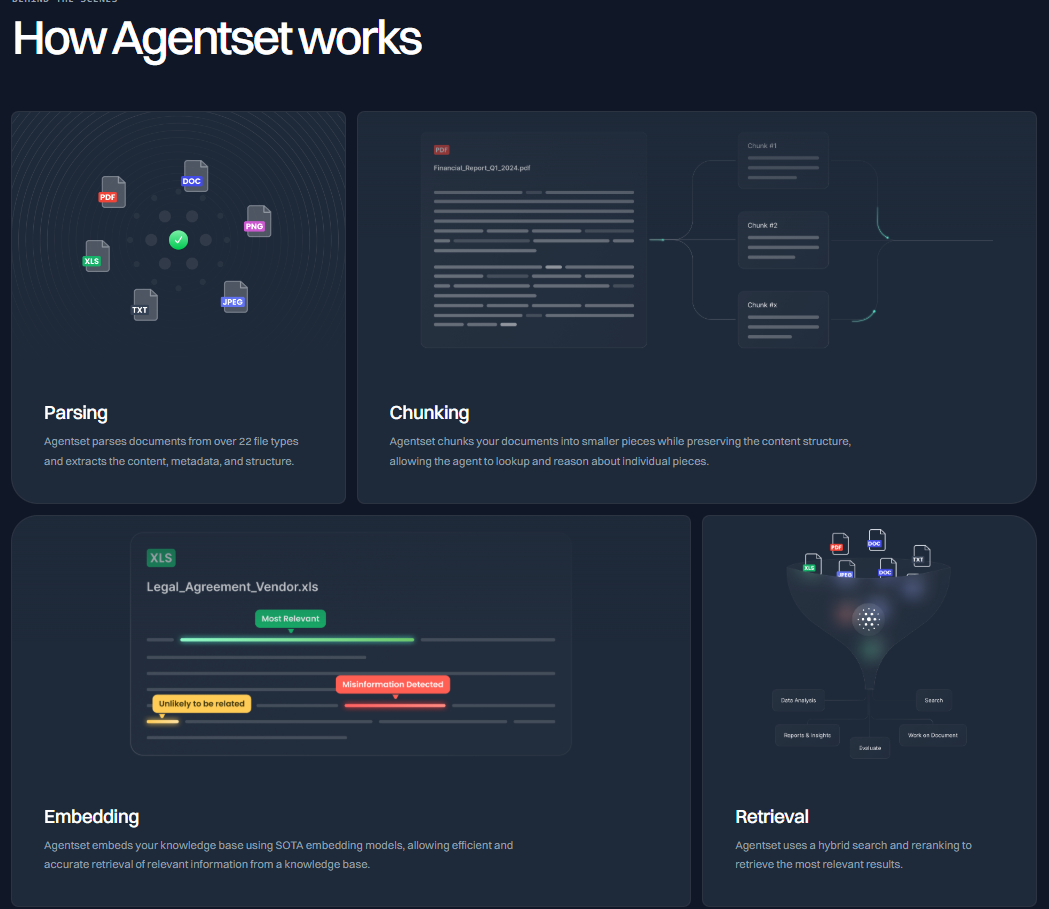
\includegraphics[width=0.8\linewidth]{images/AgentSet1.png}
    \caption{Captura de la página principal de AgentSet.}
    \label{fig:agentset}
\end{figure}

Su funcionamiento sigue un patrón ya conocido: \textit{parsing} de documentos, división en fragmentos (\textit{chunking}), generación de \textit{embeddings} y recuperación de información a partir de los mismos.  
El análisis de este y otros sistemas similares permitió identificar que no existe aún una solución empresarial ligera que funcione de manera eficiente en entornos locales sin \textit{fine-tuning}, lo cual abre la puerta a la propuesta de este trabajo.

\section{Frameworks para RAG y agentes}
La solución planteada se orienta a mejorar el rendimiento del RAG tradicional mediante técnicas avanzadas y agentes. A continuación, se presenta una comparativa de los principales frameworks empleados en proyectos de este tipo:

\begin{table}[H]
\centering
\caption{Comparativa de frameworks para RAG y agentes}
\label{tab:frameworks}
\begin{tabular}{|p{3cm}|p{4cm}|p{4cm}|p{3cm}|}
\hline
\textbf{Framework} & \textbf{Ventajas} & \textbf{Limitaciones} & \textbf{Casos de uso típicos} \\ \hline
LangChain & Amplia comunidad, gran ecosistema de integraciones & Complejidad en proyectos grandes, curva de aprendizaje elevada & Prototipado rápido, aplicaciones generales \\ \hline
LlamaIndex & Orientado a indexación y recuperación eficiente & Menor flexibilidad que LangChain & QA sobre documentos, chatbots documentales \\ \hline
LangGraph & Enfoque en agentes y grafos, facilita modularidad & Menos maduro, comunidad en crecimiento & Aplicaciones multi-agente, workflows complejos \\ \hline
Haystack & Enfoque en producción, soporta múltiples backends & Menor soporte en comunidad que LangChain & Búsqueda empresarial, pipelines NLP \\ \hline
\end{tabular}
\end{table}

Cada uno de estos frameworks presenta enfoques distintos: mientras LangChain prioriza la flexibilidad, LlamaIndex simplifica el acceso documental y LangGraph introduce el paradigma basado en grafos para mejorar el control del flujo de contexto.

\section{Bases de datos vectoriales}
Una diferencia fundamental entre implementaciones prácticas radica en cómo se almacenan y gestionan los \textit{embeddings}. Para este proyecto se analizaron las principales bases de datos vectoriales:

\begin{table}[H]
\centering
\caption{Comparativa de bases de datos vectoriales}
\label{tab:vectorDB}
\begin{tabular}{|p{3cm}|p{3cm}|p{3cm}|p{3cm}|p{3cm}|}
\hline
\textbf{Base de datos} & \textbf{Escalabilidad} & \textbf{Latencia} & \textbf{Coste} & \textbf{Integración} \\ \hline
Pinecone & Alta (SaaS, multi-región) & Baja & Pago por uso & APIs simples, integración con LangChain \\ \hline
Weaviate & Muy alta, orientada a producción & Baja & Open Source, opción SaaS & Plugins, REST/gRPC \\ \hline
FAISS & Limitada al hardware local & Muy baja (GPU optimizado) & Gratuito & Integración manual, menos amigable \\ \hline
Milvus & Escalable, soporta clusters & Media-baja & Open Source, coste en infraestructura & SDKs múltiples, alto rendimiento \\ \hline
Vespa & Altamente escalable, usado en grandes corporaciones & Media & Open Source & Más complejo de configurar \\ \hline
\end{tabular}
\end{table}

\section{Modelos de lenguaje}
No existe un único modelo estandarizado en estas aplicaciones. Según los casos analizados, se observa lo siguiente:

\begin{itemize}
    \item \textbf{Startups}: tienden a usar modelos preentrenados como ChatGPT (OpenAI) o DeepSeek, por su facilidad de integración y calidad.
    \item \textbf{Grandes empresas}: emplean modelos fine-tuneados específicamente para sus tareas, priorizando privacidad y personalización.
    \item \textbf{Modelos locales}: alternativas como LLaMA o Mistral permiten despliegues portátiles, aunque con limitaciones de rendimiento frente a modelos de API como GPT-4o o GPT-4o-mini.
\end{itemize}

De acuerdo con las pruebas realizadas, los modelos de API como ChatGPT siguen ofreciendo mejores resultados en precisión y coherencia que los modelos locales, si bien con el inconveniente del coste asociado y la dependencia de un servicio externo. En capítulos posteriores se analizan estos costes en el contexto específico del proyecto.

\section{Retos actuales y limitaciones}
A pesar del notable avance en el desarrollo y aplicación de los LLMs y sus variantes de optimización como RAG, persisten una serie de retos y limitaciones que condicionan su uso en entornos empresariales:

\begin{itemize}
    \item \textbf{Limitaciones de contexto:} aunque los modelos más recientes permiten ventanas de contexto cada vez más amplias (p.ej., GPT-4 o Claude con más de 100.000 tokens, e incluso algunos modelos experimentales con hasta un millón), la coherencia de las respuestas decae al trabajar con documentos extensos. La ampliación del contexto introduce además penalizaciones significativas en velocidad, coste y calidad de respuesta. El \textit{chunking} y la indexación no siempre garantizan una recuperación precisa; su eficacia depende del tipo de segmentación empleado y de la estructura interna de los documentos.

    \item \textbf{Alucinaciones:} los LLMs tienden a generar información inexistente o imprecisa a partir de patrones estadísticos, sin necesariamente citar fuentes verificables. En entornos regulados, esto supone riesgos legales, pérdida de confianza del usuario y costes económicos derivados de errores. Este fenómeno también puede afectar a la calidad de las respuestas en el sistema desarrollado, aunque herramientas como \textit{LettuceDetect} permiten detectar alucinaciones en las respuestas generadas.

    \item \textbf{Evaluación de resultados:} actualmente no existe un estándar robusto para medir la calidad de las respuestas, especialmente al trabajar con documentos en múltiples idiomas. Métricas como BLEU\footnote{\url{https://huggingface.co/spaces/evaluate-metric/bleu}} o ROUGE\footnote{\url{https://huggingface.co/spaces/evaluate-metric/rouge}} son útiles para evaluar la similitud léxica entre respuestas generadas y de referencia, pero no capturan la semántica ni la corrección factual. La evaluación humana, aunque más fiable, resulta subjetiva y costosa. Precisamente esta dificultad de validar respuestas automáticamente sobre documentos extensos fue uno de los detonantes del presente proyecto.

    \item \textbf{Costes computacionales:} el entrenamiento y el uso de LLMs son intensivos en recursos. Los costes asociados a las APIs comerciales (pago por token) pueden resultar prohibitivos en escenarios de gran escala, mientras que el uso de modelos locales requiere hardware dedicado con GPU de alta capacidad para obtener tiempos de respuesta aceptables.

    \item \textbf{Integración en entornos reales:} desplegar estos modelos en producción presenta retos de latencia, compatibilidad con sistemas heredados (CRMs, ERPs, bases de datos internas) y mantenimiento de \textit{pipelines} de datos. En el caso de las licitaciones públicas, la homogeneidad estructural parcial de los documentos facilita el proceso, aunque la variabilidad en formatos y codificaciones de los archivos PDF sigue representando un desafío de ingesta.
\end{itemize}

\section{Aportación del proyecto}

Del análisis precedente se desprende un ecosistema de herramientas ya consolidadas: frameworks de orquestación (LangChain, LangGraph, LlamaIndex, Haystack), bases de datos vectoriales (FAISS, ChromaDB, Pinecone, Weaviate), modelos de lenguaje locales (LLaMA, Mistral) y servicios comerciales de QA documental (Adobe, Microsoft Azure AI Document Intelligence, AgentSet). Todas estas son tecnologías existentes, no contribuciones de este trabajo. La \textbf{aportación original} reside en su combinación y adaptación específica para resolver un problema concreto —la consulta local y privada de pliegos de contratación pública— con aspectos que no están cubiertos de forma individual por ninguna de las soluciones analizadas:

\begin{itemize}
    \item \textbf{Extracción jerárquica adaptativa:} Un módulo original de segmentación de documentos PDF que reconstruye el árbol de secciones mediante hipervínculos del índice y, como mecanismo de \textit{fallback}, inferencia posicional por coordenadas X con emparejamiento difuso (\textit{fuzzy matching}). Esta lógica multiestrato, diseñada para documentos con estructuras irregulares o sin hipervínculos, no está disponible como componente reutilizable en ninguno de los frameworks analizados.

    \item \textbf{Grafo de conocimiento documental con propagación familiar de relevancia:} La representación de cada documento como un \texttt{DiGraph} de \texttt{NetworkX} con tres tipos de aristas (jerárquicas, secuenciales y semánticas) y el algoritmo de propagación familiar que eleva al Top-3 el 95\,\% de los fragmentos que el RAG vectorial puro deja fuera del Top-5. Esta capacidad de recuperar contexto estructural completo (padre $\rightarrow$ hijo) no es inherente a ninguno de los frameworks de RAG convencionales.

    \item \textbf{Agente de selección de estrategia de recuperación:} Un agente LLM especializado que clasifica cada consulta como \texttt{PARTIAL} (recuperación selectiva de fragmentos) o \texttt{FULL} (contexto completo del documento), con una tasa de acierto del 96\,\% demostrada experimentalmente. Esta decisión dinámica y adaptativa al dominio específico no es un componente estándar de los pipelines RAG analizados.

    \item \textbf{Despliegue completamente local y privado:} La integración de todos los componentes —embeddings, reranker, LLM, agentes— en un pipeline ejecutable sin conexión a internet, sin \textit{fine-tuning} ni reentrenamiento, adecuado para documentos con requisitos de confidencialidad. Esto contrasta directamente con soluciones como AgentSet, que procesa los documentos en servidores externos.

    \item \textbf{Validación empírica cuantitativa en dominio específico:} Un protocolo de evaluación con métricas automáticas (Token F1, ROUGE-L, BERTScore, RAGAS) y un estudio de ablación por componentes sobre 30 preguntas con \textit{ground truth} definido, que permite aislar y cuantificar la contribución individual de cada módulo del sistema.
\end{itemize}

En contraste con los sistemas analizados, que priorizan la escalabilidad o la facilidad de integración en arquitecturas de nube, la propuesta de este trabajo prioriza la preservación de la jerarquía documental, la soberanía del dato y la viabilidad en hardware de usuario sin modificación de modelos base.

\chapter{Motivación}\label{cap3}

En este capítulo se presentan las razones que justifican la creación de este proyecto, cuáles son sus objetivos, las etapas de desarrollo y otros datos relevantes como una estimación de presupuesto, considerando tanto el desarrollo como la puesta en práctica en un caso concreto.

Los LLMs fueron introduciéndose paulatinamente en mi vida —y posiblemente en la de cualquier estudiante—. Eran capaces de resolver dudas que un usuario podría tardar mucho tiempo en responder, generar resúmenes de contenido e incluso formular preguntas sobre el mismo. Todo ello representaba un gran valor. Sin embargo, en muchas ocasiones surgía un problema recurrente: cuando un documento era demasiado extenso, introducirlo completo en el modelo no era posible por limitaciones de contexto, y dividirlo manualmente resultaba ineficiente. El resultado eran respuestas imprecisas o incompletas.

Esta situación despertó la curiosidad por entender cómo funcionaban estos modelos y si dicho problema era realmente solucionable. En paralelo, el uso de los LLMs se expandía rápidamente entre el público general, generando un mercado cada vez más relevante. La investigación realizada permitió comprobar que, lejos de estar resuelto, se trataba de un desafío en plena evolución.

La oportunidad se concretó cuando, durante el período de prácticas en la empresa, se planteó un reto similar: trabajar con documentos de gran extensión —en concreto, licitaciones públicas— optimizando la recuperación de información y las respuestas generadas, con el objetivo de facilitar la elaboración de las memorias técnicas necesarias para concurrir a dichos procesos. El beneficio económico derivado del ahorro de tiempo del personal resultó evidente.  

En resumen, la motivación detrás de este proyecto responde a tres ejes principales:  
\begin{itemize}
    \item \textbf{Científico}: explorar y aplicar soluciones innovadoras en torno al uso de LLM en documentos extensos.  
    \item \textbf{Económico}: demostrar el potencial de ahorro de costes y optimización de procesos en entornos empresariales.  
    \item \textbf{Personal}: adquirir un conocimiento profundo de estas tecnologías y afrontar un reto de alto interés práctico.  
\end{itemize}

\section{Objetivos y etapas del proyecto}
\subsection{Objetivos}
Los principales objetivos del proyecto son:  
\begin{itemize}
    \item Desarrollar una solución personalizada al problema del contexto en los LLMs en documentos extensos, como licitaciones públicas.
    \item Comprender cómo funciona un LLM a nivel interno.
    \item Aprender y aplicar las últimas tecnologías en uso en el sector.
    \item Diseñar un sistema propio de segmentación de documentos (chunking), distinto a los clásicos.
    \item Entender y profundizar en el uso de agentes, sus librerías y aplicaciones.
    \item Explorar soluciones alternativas a las vistas en el Estado del Arte.
\end{itemize}

\subsection{Etapas}
El desarrollo del proyecto se organizó en las siguientes fases:  
\begin{itemize}
    \item \textbf{Investigación}: etapa inicial de gran importancia. Si bien contaba con conocimientos básicos, profundicé en los fundamentos: qué es un LLM, cómo funcionan los transformadores, la tokenización, etc. Posteriormente, la investigación se centró en técnicas para alimentar al modelo con información contextualizada, como RAG y GraphRAG. Para ello se emplearon fuentes diversas, desde foros oficiales hasta tutoriales prácticos.  
    \item \textbf{Diseño}: desde un inicio se optó por una arquitectura en tres capas:  
        \begin{enumerate}
            \item Capa de agentes, responsables de la toma de decisiones.  
            \item Capa de segmentación de documentos, encargada de dividir en chunks limpios y eficientes en número de tokens.  
            \item Capa de lógica del modelo, que realiza las ponderaciones y devuelve al usuario una respuesta coherente y fundamentada.  
        \end{enumerate}
    \item \textbf{Implementación}: se afrontaron retos técnicos como incompatibilidades entre librerías, pruebas con diferentes métodos y las imprecisiones frecuentes en modelos locales.  
    \item \textbf{Validación}: se realizaron pruebas sobre el \textit{dataset} de documentos descrito en el Capítulo~\ref{cap7}, combinando un estudio de ablación por componentes con la métrica de precisión de recuperación P@3 sobre un conjunto de 30 preguntas con respuesta de referencia conocida. En el entorno empresarial se empleó adicionalmente la herramienta \textit{LettuceDetect} para la detección de alucinaciones en las respuestas generadas, así como validaciones empíricas con casos de uso reales.
\end{itemize}

\section{Recursos utilizados}
Para el desarrollo del proyecto se emplearon los siguientes recursos:  

\begin{itemize}
    \item \textbf{Software}: se utilizó Python como lenguaje de programación, junto con librerías clave como:
    \begin{itemize}
        \item \texttt{rank\_bm25} (BM25Okapi) para recuperación de información.  
        \item \texttt{networkx} para la representación y manipulación de grafos.  
        \item \texttt{matplotlib} para la visualización.  
        \item \texttt{sentence\_transformers} y \texttt{scikit-learn} para embeddings y métricas de similitud.  
        \item \texttt{ollama} y \texttt{tiktoken} para la gestión de modelos y conteo de tokens.  
        \item \texttt{thefuzz} para comparación de cadenas.  
        \item \texttt{langchain} y \texttt{CrossEncoder} para operaciones avanzadas en RAG.  .  
    \end{itemize}

    \item \textbf{Hardware}: se trabajó principalmente en un portátil proporcionado por la empresa (MSI Cyborg, 32 GB RAM y GPU dedicada), que, si bien es un dispositivo portátil, permite ejecutar modelos locales de hasta 8--13B parámetros con aceleración CUDA.

    \item \textbf{Recursos humanos}: el trabajo fue realizado de manera individual, con el apoyo de un \textit{Senior} con conocimientos en IA, con reuniones casi diarias para la supervisión y resolución de problemas.  
\end{itemize}

\section{Caso de negocio}
Este apartado expone la aplicabilidad y justificación del proyecto en un entorno real.  

\subsection{Agentes implicados en el proyecto}
\begin{itemize}
    \item \textbf{Beneficiarios directos}: la empresa en la que se desarrolló el proyecto, al mejorar la eficiencia en el manejo de documentos extensos como licitaciones públicas. Su implementación se encuentra en fase de piloto, prevista para su puesta en producción una vez se reactive el mercado de consultoría tras el período estival.
    \item \textbf{Usuarios finales}: personal de la empresa que necesita consultar información en grandes volúmenes de texto y elaborar las memorias técnicas para concurrir a licitaciones, así como cualquier otro rol que pudiera beneficiarse de una herramienta de consulta documental.
    \item \textbf{Otros interesados}: investigadores interesados en la optimización de sistemas RAG y en el uso de GraphRAG como enfoque alternativo, así como potenciales clientes de sectores con necesidades documentales similares.
\end{itemize}

\subsection{Presupuesto}
La siguiente tabla resume una estimación de los costes asociados al proyecto:

\begin{table}[H]
\centering
\small
\begin{tabularx}{\textwidth}{|l|c|>{\raggedright\arraybackslash}X|}
\hline
\textbf{Concepto} & \textbf{Coste estimado (€)} & \textbf{Observaciones} \\ \hline
Hardware (portátil) & 1.200 & Proporcionado por la empresa \\ \hline
Software & 200 & Librerías open source, salvo costes puntuales \\ \hline
Horas de trabajo (160 h aprox.) & 2.660 & 20 h/semana durante 2 meses, tarifa Junior (Usando el coste a la empresa, no lo que cobra el trabajador) \\ \hline
Costes adicionales (cloud, API) & 0,50 & Cada consulta +- 0,01 €, uso puntual \\ \hline
\textbf{Total estimado} & \textbf{4.060,50} &  \\ \hline
\end{tabularx}
\caption{Estimación de presupuesto del proyecto.}
\label{tab:presupuesto}
\end{table}

Se entrará más en los gastos de la API en el capítulo de implementación, pero muchas de las consultas no superaban el céntimo de euro por petición.  
En cuanto a las horas de trabajo, el coste se estimó a partir de las horas invertidas (20 semanales durante aproximadamente 2 meses) y multiplicado por un sueldo estándar de \textit{Developer Junior} en coste a la empresa. Este cálculo es meramente orientativo, ya que una persona trabajando a jornada completa y con mayor experiencia podría reducir los tiempos y, por tanto, los costes, en función del nivel salarial correspondiente.


\begin{table}[H]
\centering
\begin{tabularx}{\textwidth}{|l|X|X|}
\hline
\textbf{Concepto} & \textbf{Coste mensual estimado (€)} & \textbf{Observaciones} \\ \hline
Servidor físico (GPU 24--48 GB VRAM, 128 GB RAM) & 4.800 & Precio de adquisición, amortizado a 3 años \\ \hline
Electricidad & 120 & Consumo medio 400 W en uso continuo \\ \hline
Mantenimiento (hardware/software) & 50 & Reemplazos, soporte, licencias menores \\ \hline
\textbf{Total mensual} & \textbf{500} & Incluye amortización del hardware \\ \hline
\end{tabularx}
\caption{Estimación de costes mensuales para mantener un servidor con un modelo LLM local.}
\label{tab:servidor}
\end{table}

En este cálculo se supone la adquisición de una máquina capaz de albergar un modelo de entre 7B y 13B parámetros (ej. NVIDIA RTX A6000 o similar con 48 GB de VRAM). Se amortiza el coste del hardware (aprox. 4.800 €) en un periodo de 3 años, resultando unos 400 € mensuales.  
A esto se añade el coste eléctrico (400 W de consumo medio, 24/7, con un precio aproximado de 0,25 €/kWh) y una partida para mantenimiento preventivo y correctivo.  
El coste total mensual ronda los \textbf{500 €}, lo cual permite comparar la viabilidad frente a soluciones en la nube. Nótese que, según las pruebas realizadas, es posible que se requieran modelos con más parámetros para casos de uso más exigentes, lo que incrementaría el coste. De nuevo, este cálculo es meramente orientativo.



\subsection{Impacto}
El impacto del proyecto puede resumirse en los siguientes puntos:  
\begin{itemize}
    \item \textbf{Productividad}: reducción significativa del tiempo necesario para consultar documentos extensos.  
    \item \textbf{Eficiencia}: posibilidad de automatizar tareas de análisis documental, liberando recursos humanos para labores de mayor valor añadido.  
    \item \textbf{Aplicaciones futuras}: escalabilidad hacia otros tipos de documentos o incluso integración con sistemas empresariales más amplios.  
    \item \textbf{Impacto académico}: contribución al estudio de técnicas alternativas al RAG tradicional, con valor tanto práctico como científico.  
\end{itemize}
